% Created by tikzDevice version 0.12.3.1 on 2022-09-20 12:45:22
% !TEX encoding = UTF-8 Unicode
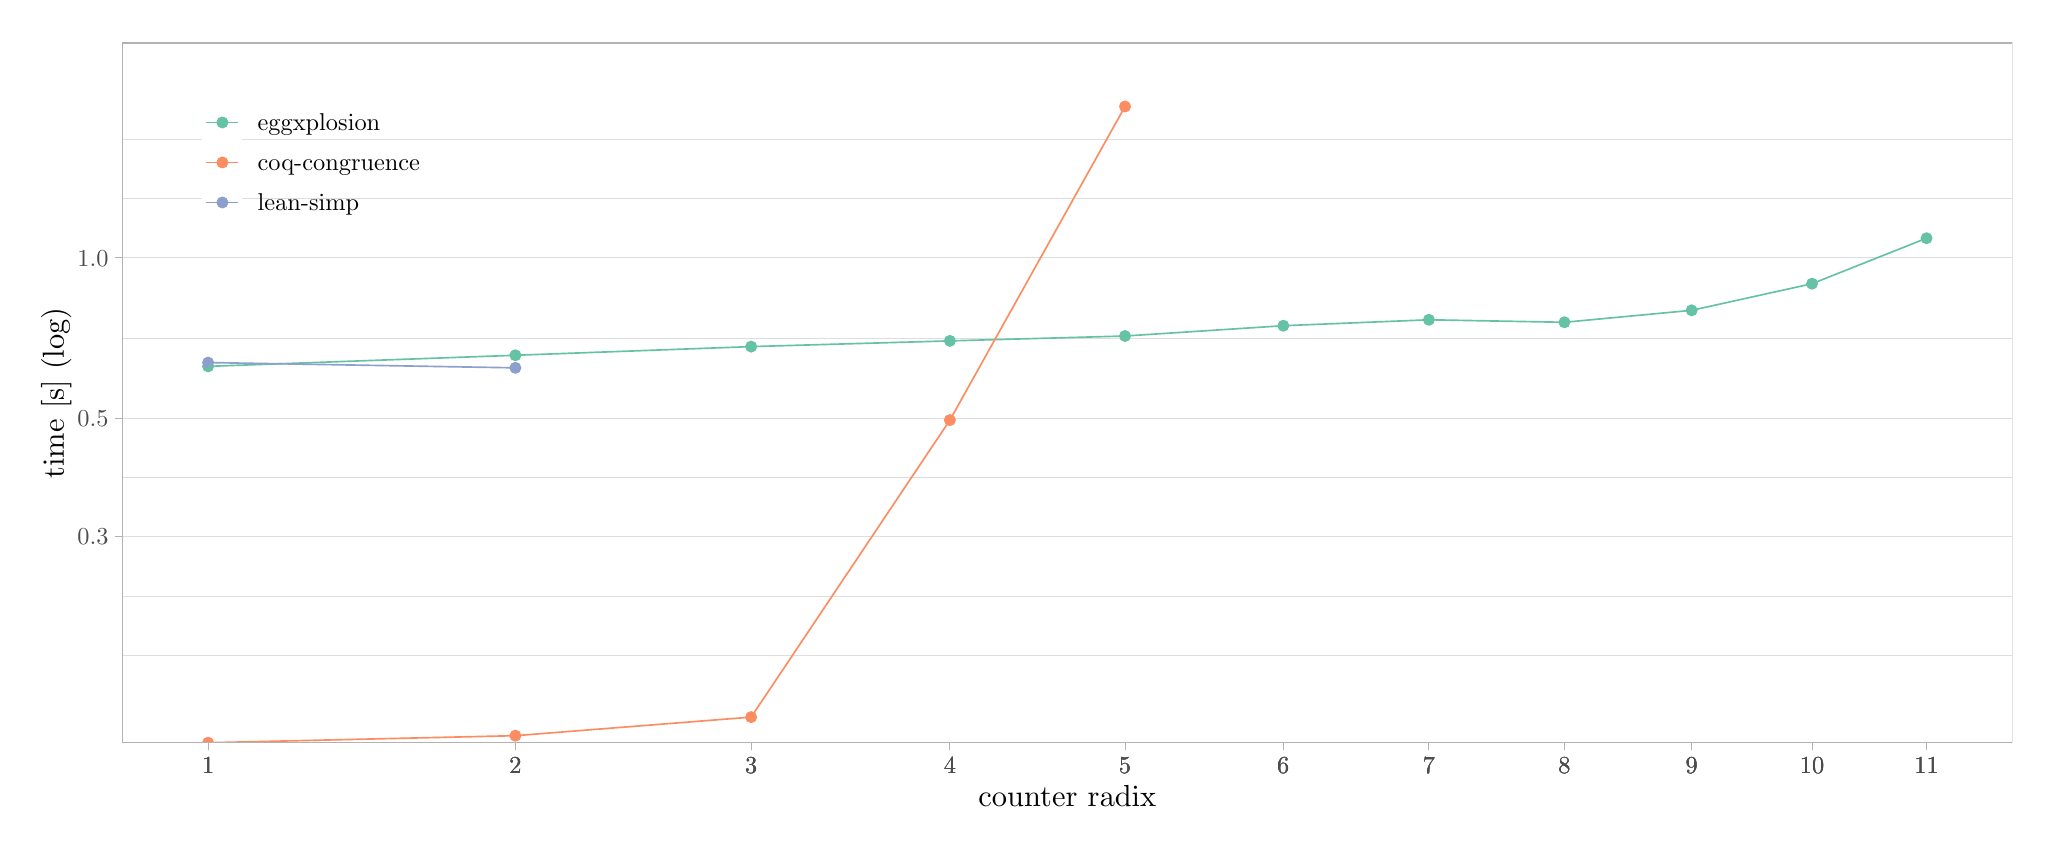
\begin{tikzpicture}[x=1pt,y=1pt]
\definecolor{fillColor}{RGB}{255,255,255}
\path[use as bounding box,fill=fillColor,fill opacity=0.00] (0,0) rectangle (722.70,289.08);
\begin{scope}
\path[clip] (  0.00,  0.00) rectangle (722.70,289.08);
\definecolor{drawColor}{RGB}{255,255,255}
\definecolor{fillColor}{RGB}{255,255,255}

\path[draw=drawColor,line width= 0.6pt,line join=round,line cap=round,fill=fillColor] (  0.00,  0.00) rectangle (722.70,289.08);
\end{scope}
\begin{scope}
\path[clip] ( 34.16, 30.69) rectangle (717.20,283.58);
\definecolor{fillColor}{RGB}{255,255,255}

\path[fill=fillColor] ( 34.16, 30.69) rectangle (717.20,283.58);
\definecolor{drawColor}{gray}{0.87}

\path[draw=drawColor,line width= 0.1pt,line join=round] ( 34.16, 62.43) --
	(717.20, 62.43);

\path[draw=drawColor,line width= 0.1pt,line join=round] ( 34.16, 83.81) --
	(717.20, 83.81);

\path[draw=drawColor,line width= 0.1pt,line join=round] ( 34.16,126.56) --
	(717.20,126.56);

\path[draw=drawColor,line width= 0.1pt,line join=round] ( 34.16,176.95) --
	(717.20,176.95);

\path[draw=drawColor,line width= 0.1pt,line join=round] ( 34.16,227.33) --
	(717.20,227.33);

\path[draw=drawColor,line width= 0.1pt,line join=round] ( 34.16,248.71) --
	(717.20,248.71);

\path[draw=drawColor,line width= 0.3pt,line join=round] ( 34.16,105.19) --
	(717.20,105.19);

\path[draw=drawColor,line width= 0.3pt,line join=round] ( 34.16,147.94) --
	(717.20,147.94);

\path[draw=drawColor,line width= 0.3pt,line join=round] ( 34.16,205.95) --
	(717.20,205.95);
\definecolor{drawColor}{RGB}{102,194,165}
\definecolor{fillColor}{RGB}{102,194,165}

\path[draw=drawColor,line width= 0.4pt,line join=round,line cap=round,fill=fillColor] ( 65.20,166.69) circle (  1.96);
\definecolor{drawColor}{RGB}{141,160,203}
\definecolor{fillColor}{RGB}{141,160,203}

\path[draw=drawColor,line width= 0.4pt,line join=round,line cap=round,fill=fillColor] ( 65.20,168.07) circle (  1.96);
\definecolor{drawColor}{RGB}{252,141,98}
\definecolor{fillColor}{RGB}{252,141,98}

\path[draw=drawColor,line width= 0.4pt,line join=round,line cap=round,fill=fillColor] ( 65.20, 30.69) circle (  1.96);
\definecolor{drawColor}{RGB}{102,194,165}
\definecolor{fillColor}{RGB}{102,194,165}

\path[draw=drawColor,line width= 0.4pt,line join=round,line cap=round,fill=fillColor] (176.23,170.70) circle (  1.96);
\definecolor{drawColor}{RGB}{141,160,203}
\definecolor{fillColor}{RGB}{141,160,203}

\path[draw=drawColor,line width= 0.4pt,line join=round,line cap=round,fill=fillColor] (176.23,166.16) circle (  1.96);
\definecolor{drawColor}{RGB}{252,141,98}
\definecolor{fillColor}{RGB}{252,141,98}

\path[draw=drawColor,line width= 0.4pt,line join=round,line cap=round,fill=fillColor] (176.23, 33.24) circle (  1.96);
\definecolor{drawColor}{RGB}{102,194,165}
\definecolor{fillColor}{RGB}{102,194,165}

\path[draw=drawColor,line width= 0.4pt,line join=round,line cap=round,fill=fillColor] (261.42,173.83) circle (  1.96);
\definecolor{drawColor}{RGB}{252,141,98}
\definecolor{fillColor}{RGB}{252,141,98}

\path[draw=drawColor,line width= 0.4pt,line join=round,line cap=round,fill=fillColor] (261.42, 39.95) circle (  1.96);
\definecolor{drawColor}{RGB}{102,194,165}
\definecolor{fillColor}{RGB}{102,194,165}

\path[draw=drawColor,line width= 0.4pt,line join=round,line cap=round,fill=fillColor] (333.24,175.90) circle (  1.96);
\definecolor{drawColor}{RGB}{252,141,98}
\definecolor{fillColor}{RGB}{252,141,98}

\path[draw=drawColor,line width= 0.4pt,line join=round,line cap=round,fill=fillColor] (333.24,147.27) circle (  1.96);
\definecolor{drawColor}{RGB}{102,194,165}
\definecolor{fillColor}{RGB}{102,194,165}

\path[draw=drawColor,line width= 0.4pt,line join=round,line cap=round,fill=fillColor] (396.52,177.66) circle (  1.96);
\definecolor{drawColor}{RGB}{252,141,98}
\definecolor{fillColor}{RGB}{252,141,98}

\path[draw=drawColor,line width= 0.4pt,line join=round,line cap=round,fill=fillColor] (396.52,260.59) circle (  1.96);
\definecolor{drawColor}{RGB}{102,194,165}
\definecolor{fillColor}{RGB}{102,194,165}

\path[draw=drawColor,line width= 0.4pt,line join=round,line cap=round,fill=fillColor] (453.73,181.38) circle (  1.96);

\path[draw=drawColor,line width= 0.4pt,line join=round,line cap=round,fill=fillColor] (506.33,183.52) circle (  1.96);

\path[draw=drawColor,line width= 0.4pt,line join=round,line cap=round,fill=fillColor] (555.30,182.62) circle (  1.96);

\path[draw=drawColor,line width= 0.4pt,line join=round,line cap=round,fill=fillColor] (601.28,186.94) circle (  1.96);

\path[draw=drawColor,line width= 0.4pt,line join=round,line cap=round,fill=fillColor] (644.78,196.56) circle (  1.96);

\path[draw=drawColor,line width= 0.4pt,line join=round,line cap=round,fill=fillColor] (686.15,213.00) circle (  1.96);

\path[draw=drawColor,line width= 0.6pt,line join=round] ( 65.20,166.69) --
	(176.23,170.70) --
	(261.42,173.83) --
	(333.24,175.90) --
	(396.52,177.66) --
	(453.73,181.38) --
	(506.33,183.52) --
	(555.30,182.62) --
	(601.28,186.94) --
	(644.78,196.56) --
	(686.15,213.00);
\definecolor{drawColor}{RGB}{252,141,98}

\path[draw=drawColor,line width= 0.6pt,line join=round] ( 65.20, 30.69) --
	(176.23, 33.24) --
	(261.42, 39.95) --
	(333.24,147.27) --
	(396.52,260.59);
\definecolor{drawColor}{RGB}{141,160,203}

\path[draw=drawColor,line width= 0.6pt,line join=round] ( 65.20,168.07) --
	(176.23,166.16);
\definecolor{drawColor}{gray}{0.70}

\path[draw=drawColor,line width= 0.6pt,line join=round,line cap=round] ( 34.16, 30.69) rectangle (717.20,283.58);
\end{scope}
\begin{scope}
\path[clip] (  0.00,  0.00) rectangle (722.70,289.08);
\definecolor{drawColor}{gray}{0.30}

\node[text=drawColor,anchor=base east,inner sep=0pt, outer sep=0pt, scale=  0.88] at ( 29.21,102.16) {0.3};

\node[text=drawColor,anchor=base east,inner sep=0pt, outer sep=0pt, scale=  0.88] at ( 29.21,144.91) {0.5};

\node[text=drawColor,anchor=base east,inner sep=0pt, outer sep=0pt, scale=  0.88] at ( 29.21,202.92) {1.0};
\end{scope}
\begin{scope}
\path[clip] (  0.00,  0.00) rectangle (722.70,289.08);
\definecolor{drawColor}{gray}{0.70}

\path[draw=drawColor,line width= 0.3pt,line join=round] ( 31.41,105.19) --
	( 34.16,105.19);

\path[draw=drawColor,line width= 0.3pt,line join=round] ( 31.41,147.94) --
	( 34.16,147.94);

\path[draw=drawColor,line width= 0.3pt,line join=round] ( 31.41,205.95) --
	( 34.16,205.95);
\end{scope}
\begin{scope}
\path[clip] (  0.00,  0.00) rectangle (722.70,289.08);
\definecolor{drawColor}{gray}{0.70}

\path[draw=drawColor,line width= 0.3pt,line join=round] ( 65.20, 27.94) --
	( 65.20, 30.69);

\path[draw=drawColor,line width= 0.3pt,line join=round] ( 65.20, 27.94) --
	( 65.20, 30.69);

\path[draw=drawColor,line width= 0.3pt,line join=round] ( 65.20, 27.94) --
	( 65.20, 30.69);

\path[draw=drawColor,line width= 0.3pt,line join=round] (176.23, 27.94) --
	(176.23, 30.69);

\path[draw=drawColor,line width= 0.3pt,line join=round] (176.23, 27.94) --
	(176.23, 30.69);

\path[draw=drawColor,line width= 0.3pt,line join=round] (176.23, 27.94) --
	(176.23, 30.69);

\path[draw=drawColor,line width= 0.3pt,line join=round] (261.42, 27.94) --
	(261.42, 30.69);

\path[draw=drawColor,line width= 0.3pt,line join=round] (261.42, 27.94) --
	(261.42, 30.69);

\path[draw=drawColor,line width= 0.3pt,line join=round] (261.42, 27.94) --
	(261.42, 30.69);

\path[draw=drawColor,line width= 0.3pt,line join=round] (333.24, 27.94) --
	(333.24, 30.69);

\path[draw=drawColor,line width= 0.3pt,line join=round] (333.24, 27.94) --
	(333.24, 30.69);

\path[draw=drawColor,line width= 0.3pt,line join=round] (333.24, 27.94) --
	(333.24, 30.69);

\path[draw=drawColor,line width= 0.3pt,line join=round] (396.52, 27.94) --
	(396.52, 30.69);

\path[draw=drawColor,line width= 0.3pt,line join=round] (396.52, 27.94) --
	(396.52, 30.69);

\path[draw=drawColor,line width= 0.3pt,line join=round] (396.52, 27.94) --
	(396.52, 30.69);

\path[draw=drawColor,line width= 0.3pt,line join=round] (453.73, 27.94) --
	(453.73, 30.69);

\path[draw=drawColor,line width= 0.3pt,line join=round] (453.73, 27.94) --
	(453.73, 30.69);

\path[draw=drawColor,line width= 0.3pt,line join=round] (453.73, 27.94) --
	(453.73, 30.69);

\path[draw=drawColor,line width= 0.3pt,line join=round] (506.33, 27.94) --
	(506.33, 30.69);

\path[draw=drawColor,line width= 0.3pt,line join=round] (506.33, 27.94) --
	(506.33, 30.69);

\path[draw=drawColor,line width= 0.3pt,line join=round] (506.33, 27.94) --
	(506.33, 30.69);

\path[draw=drawColor,line width= 0.3pt,line join=round] (555.30, 27.94) --
	(555.30, 30.69);

\path[draw=drawColor,line width= 0.3pt,line join=round] (555.30, 27.94) --
	(555.30, 30.69);

\path[draw=drawColor,line width= 0.3pt,line join=round] (555.30, 27.94) --
	(555.30, 30.69);

\path[draw=drawColor,line width= 0.3pt,line join=round] (601.28, 27.94) --
	(601.28, 30.69);

\path[draw=drawColor,line width= 0.3pt,line join=round] (601.28, 27.94) --
	(601.28, 30.69);

\path[draw=drawColor,line width= 0.3pt,line join=round] (601.28, 27.94) --
	(601.28, 30.69);

\path[draw=drawColor,line width= 0.3pt,line join=round] (644.78, 27.94) --
	(644.78, 30.69);

\path[draw=drawColor,line width= 0.3pt,line join=round] (644.78, 27.94) --
	(644.78, 30.69);

\path[draw=drawColor,line width= 0.3pt,line join=round] (644.78, 27.94) --
	(644.78, 30.69);

\path[draw=drawColor,line width= 0.3pt,line join=round] (686.15, 27.94) --
	(686.15, 30.69);

\path[draw=drawColor,line width= 0.3pt,line join=round] (686.15, 27.94) --
	(686.15, 30.69);

\path[draw=drawColor,line width= 0.3pt,line join=round] (686.15, 27.94) --
	(686.15, 30.69);
\end{scope}
\begin{scope}
\path[clip] (  0.00,  0.00) rectangle (722.70,289.08);
\definecolor{drawColor}{gray}{0.30}

\node[text=drawColor,anchor=base,inner sep=0pt, outer sep=0pt, scale=  0.88] at ( 65.20, 19.68) {1};

\node[text=drawColor,anchor=base,inner sep=0pt, outer sep=0pt, scale=  0.88] at ( 65.20, 19.68) {1};

\node[text=drawColor,anchor=base,inner sep=0pt, outer sep=0pt, scale=  0.88] at ( 65.20, 19.68) {1};

\node[text=drawColor,anchor=base,inner sep=0pt, outer sep=0pt, scale=  0.88] at (176.23, 19.68) {2};

\node[text=drawColor,anchor=base,inner sep=0pt, outer sep=0pt, scale=  0.88] at (176.23, 19.68) {2};

\node[text=drawColor,anchor=base,inner sep=0pt, outer sep=0pt, scale=  0.88] at (176.23, 19.68) {2};

\node[text=drawColor,anchor=base,inner sep=0pt, outer sep=0pt, scale=  0.88] at (261.42, 19.68) {3};

\node[text=drawColor,anchor=base,inner sep=0pt, outer sep=0pt, scale=  0.88] at (261.42, 19.68) {3};

\node[text=drawColor,anchor=base,inner sep=0pt, outer sep=0pt, scale=  0.88] at (261.42, 19.68) {3};

\node[text=drawColor,anchor=base,inner sep=0pt, outer sep=0pt, scale=  0.88] at (333.24, 19.68) {4};

\node[text=drawColor,anchor=base,inner sep=0pt, outer sep=0pt, scale=  0.88] at (333.24, 19.68) {4};

\node[text=drawColor,anchor=base,inner sep=0pt, outer sep=0pt, scale=  0.88] at (333.24, 19.68) {4};

\node[text=drawColor,anchor=base,inner sep=0pt, outer sep=0pt, scale=  0.88] at (396.52, 19.68) {5};

\node[text=drawColor,anchor=base,inner sep=0pt, outer sep=0pt, scale=  0.88] at (396.52, 19.68) {5};

\node[text=drawColor,anchor=base,inner sep=0pt, outer sep=0pt, scale=  0.88] at (396.52, 19.68) {5};

\node[text=drawColor,anchor=base,inner sep=0pt, outer sep=0pt, scale=  0.88] at (453.73, 19.68) {6};

\node[text=drawColor,anchor=base,inner sep=0pt, outer sep=0pt, scale=  0.88] at (453.73, 19.68) {6};

\node[text=drawColor,anchor=base,inner sep=0pt, outer sep=0pt, scale=  0.88] at (453.73, 19.68) {6};

\node[text=drawColor,anchor=base,inner sep=0pt, outer sep=0pt, scale=  0.88] at (506.33, 19.68) {7};

\node[text=drawColor,anchor=base,inner sep=0pt, outer sep=0pt, scale=  0.88] at (506.33, 19.68) {7};

\node[text=drawColor,anchor=base,inner sep=0pt, outer sep=0pt, scale=  0.88] at (506.33, 19.68) {7};

\node[text=drawColor,anchor=base,inner sep=0pt, outer sep=0pt, scale=  0.88] at (555.30, 19.68) {8};

\node[text=drawColor,anchor=base,inner sep=0pt, outer sep=0pt, scale=  0.88] at (555.30, 19.68) {8};

\node[text=drawColor,anchor=base,inner sep=0pt, outer sep=0pt, scale=  0.88] at (555.30, 19.68) {8};

\node[text=drawColor,anchor=base,inner sep=0pt, outer sep=0pt, scale=  0.88] at (601.28, 19.68) {9};

\node[text=drawColor,anchor=base,inner sep=0pt, outer sep=0pt, scale=  0.88] at (601.28, 19.68) {9};

\node[text=drawColor,anchor=base,inner sep=0pt, outer sep=0pt, scale=  0.88] at (601.28, 19.68) {9};

\node[text=drawColor,anchor=base,inner sep=0pt, outer sep=0pt, scale=  0.88] at (644.78, 19.68) {10};

\node[text=drawColor,anchor=base,inner sep=0pt, outer sep=0pt, scale=  0.88] at (644.78, 19.68) {10};

\node[text=drawColor,anchor=base,inner sep=0pt, outer sep=0pt, scale=  0.88] at (644.78, 19.68) {10};

\node[text=drawColor,anchor=base,inner sep=0pt, outer sep=0pt, scale=  0.88] at (686.15, 19.68) {11};

\node[text=drawColor,anchor=base,inner sep=0pt, outer sep=0pt, scale=  0.88] at (686.15, 19.68) {11};

\node[text=drawColor,anchor=base,inner sep=0pt, outer sep=0pt, scale=  0.88] at (686.15, 19.68) {11};
\end{scope}
\begin{scope}
\path[clip] (  0.00,  0.00) rectangle (722.70,289.08);
\definecolor{drawColor}{RGB}{0,0,0}

\node[text=drawColor,anchor=base,inner sep=0pt, outer sep=0pt, scale=  1.10] at (375.68,  7.64) {counter radix};
\end{scope}
\begin{scope}
\path[clip] (  0.00,  0.00) rectangle (722.70,289.08);
\definecolor{drawColor}{RGB}{0,0,0}

\node[text=drawColor,rotate= 90.00,anchor=base,inner sep=0pt, outer sep=0pt, scale=  1.10] at ( 13.08,157.13) {time [s] (log)};
\end{scope}
\begin{scope}
\path[clip] (  0.00,  0.00) rectangle (722.70,289.08);
\definecolor{fillColor}{RGB}{255,255,255}

\path[fill=fillColor] ( 63.14,247.59) rectangle ( 77.60,262.05);
\end{scope}
\begin{scope}
\path[clip] (  0.00,  0.00) rectangle (722.70,289.08);
\definecolor{drawColor}{RGB}{102,194,165}
\definecolor{fillColor}{RGB}{102,194,165}

\path[draw=drawColor,line width= 0.4pt,line join=round,line cap=round,fill=fillColor] ( 70.37,254.82) circle (  1.96);
\end{scope}
\begin{scope}
\path[clip] (  0.00,  0.00) rectangle (722.70,289.08);
\definecolor{drawColor}{RGB}{102,194,165}

\path[draw=drawColor,line width= 0.6pt,line join=round] ( 64.59,254.82) -- ( 76.15,254.82);
\end{scope}
\begin{scope}
\path[clip] (  0.00,  0.00) rectangle (722.70,289.08);
\definecolor{fillColor}{RGB}{255,255,255}

\path[fill=fillColor] ( 63.14,233.14) rectangle ( 77.60,247.59);
\end{scope}
\begin{scope}
\path[clip] (  0.00,  0.00) rectangle (722.70,289.08);
\definecolor{drawColor}{RGB}{252,141,98}
\definecolor{fillColor}{RGB}{252,141,98}

\path[draw=drawColor,line width= 0.4pt,line join=round,line cap=round,fill=fillColor] ( 70.37,240.37) circle (  1.96);
\end{scope}
\begin{scope}
\path[clip] (  0.00,  0.00) rectangle (722.70,289.08);
\definecolor{drawColor}{RGB}{252,141,98}

\path[draw=drawColor,line width= 0.6pt,line join=round] ( 64.59,240.37) -- ( 76.15,240.37);
\end{scope}
\begin{scope}
\path[clip] (  0.00,  0.00) rectangle (722.70,289.08);
\definecolor{fillColor}{RGB}{255,255,255}

\path[fill=fillColor] ( 63.14,218.69) rectangle ( 77.60,233.14);
\end{scope}
\begin{scope}
\path[clip] (  0.00,  0.00) rectangle (722.70,289.08);
\definecolor{drawColor}{RGB}{141,160,203}
\definecolor{fillColor}{RGB}{141,160,203}

\path[draw=drawColor,line width= 0.4pt,line join=round,line cap=round,fill=fillColor] ( 70.37,225.91) circle (  1.96);
\end{scope}
\begin{scope}
\path[clip] (  0.00,  0.00) rectangle (722.70,289.08);
\definecolor{drawColor}{RGB}{141,160,203}

\path[draw=drawColor,line width= 0.6pt,line join=round] ( 64.59,225.91) -- ( 76.15,225.91);
\end{scope}
\begin{scope}
\path[clip] (  0.00,  0.00) rectangle (722.70,289.08);
\definecolor{drawColor}{RGB}{0,0,0}

\node[text=drawColor,anchor=base west,inner sep=0pt, outer sep=0pt, scale=  0.88] at ( 83.10,251.79) {eggxplosion};
\end{scope}
\begin{scope}
\path[clip] (  0.00,  0.00) rectangle (722.70,289.08);
\definecolor{drawColor}{RGB}{0,0,0}

\node[text=drawColor,anchor=base west,inner sep=0pt, outer sep=0pt, scale=  0.88] at ( 83.10,237.34) {coq-congruence};
\end{scope}
\begin{scope}
\path[clip] (  0.00,  0.00) rectangle (722.70,289.08);
\definecolor{drawColor}{RGB}{0,0,0}

\node[text=drawColor,anchor=base west,inner sep=0pt, outer sep=0pt, scale=  0.88] at ( 83.10,222.88) {lean-simp};
\end{scope}
\end{tikzpicture}
